\chapter{Prallel Implementation}
 \label{chap:pi}
 \section{Introduction}
\hspace{10mm}In the parallel implementation the unique NEC numbering, CVS generation in data graph, and checking whether the query graph exists in the subgraph are done in GPU. The combination generation is done in CPU.

\section{Algorithm}
 \label{sec:al}
 
\begin{breakablealgorithm}[H]
\caption{Parallel $Turbo_{iso}$}
%\label{Graph Isomorphism}
\textbf{Procedure}: NECGen()\\
Parallel NEC generation on each node.\\
\textbf{Input}: Query Graph $Q$.\\
\textbf{Output}: NEC.\\
\begin{algorithmic}
\item \begin{enumerate}
\item repeat until all nodes got NEC
\item Run parallel on all nodes
\begin{enumerate}
\item running on node v
\item iterate over all neighbors of vertex v
\item if not all neighbors have NEC return
\item find the hash of neighborhood.set it hash location to 1.
\end{enumerate}
\item assign unique numbering to all 1's in the hash array
\item Run parallel on all nodes
\begin{enumerate}
\item running on node v
\item iterate over all neighbors of vertex v
\item if not all neighbors have NEC return
\item find the hash of neighborhood.Find the unique NEC in hash location
\item assign it to the vertex
\end{enumerate}
\end{enumerate}
\end{algorithmic}
\textbf{Procedure}: CVSGen()\\
Parallel CVS generation for each NEC.\\
\textbf{Input}: Data Graph $Q$,NEC.\\
\textbf{Output}: CVS.\\
\begin{algorithmic}
\item \begin{enumerate}
\item all nodes in data graph is in NEC 1
\item for each NEC from 2 to last
\item Run parallel on all nodes
\begin{enumerate}
\item running on node v
\item iterate over all neighbors of vertex v.
\item check the existence of the neighbourhood of NEC on the node v.
\item if found set the flag 1.
\end{enumerate}
\end{enumerate}
\end{algorithmic}

\textbf{Procedure}: PermandComb()\\
Parallel check all possible permutations and combinations.\\
\textbf{Input}: Data Graph $D$, Query Graph $Q$, Current vertex index(i),Possibilities(P),MaximumPossibilities(MP)\\
\textbf{Output}: Mapping of nodes from query graph to data graph.\\
\begin{algorithmic}
\item \begin{enumerate}
\item if i= $|V(q)|$
\item Report all values in P and return
\item else
 \begin{enumerate}
\item find u,the NEC of the vertex
\item Multiply P with CVSGen(u)
\item while $P >= MP$
 \begin{enumerate}
\item call CheckMap() on MP elements of P
\item call Exclusive-scan on Checkmap output
\item Save valid possibilies to newP 
\item P-=MP (numbers)
\end{enumerate}
\item move newP to P.
\end{enumerate}
\end{enumerate}
\end{algorithmic}
\textbf{Procedure}: CheckMap()\\
Parallel check of existence of query graph.\\
\textbf{Input}: Data Graph $D$,Map m,Query Graph $Q$,till vertex $v$ in query graph.\\
\textbf{Output}: true/false.\\
\begin{algorithmic}
\item \begin{enumerate}
\item running on all nodes u if $u<=v$.
\item iterate over all neighbors of vertex u.
\item check the existence of all edges in data graph corresponding to one in query graph.
\item if not all edges present set false.
\end{enumerate}

\end{algorithmic}
\end{breakablealgorithm}

\hspace{10mm}The procedure $NECGen$ gives unique ids to one tree in the query graph similar to Figure 4. We do a level order traversal on the tree. So at some nodes all its children may not have NEC given we process those nodes in the next iterations. The step 2 finds the neighbourhoods that can be processed at the current iteration and finds a hash of the neighbourhood. To these unique hashes we assign numbering by scan algorithm. Then these numberings are assigned back to each nodes.
	
\hspace{10mm} The procedure $CVSGen $ finds the candidates for a particular NEC. They check on each node on datagraph and checks the neighbouring nodes for matching negibours of the particular NEC in querygraph.

\hspace{10mm} The procedure $PermandComb$ finds all possibilites of the query graph. For eachvertex of query graph it finds all possibilites(current possibilities x CvsGen(u)). If the possibilies is more than we can store(MP), $CheckMap$ is called on all current possibilities and the wrong ones are removed. This will make the P <MP. At last when i= $|V(q)|$, P has all valid possibilites. The procedure $CheckMap$ checks the existence on non tree edges are actually present in the current 	mapping. If $CheckMap$ retruns true it is reported as a correct mapping.
\section{Inferences}
\hspace{10mm}The parallel version needs to store the mapped NEC for each node in the data graph. This is asking for a space of $O(n*N(q))$ where $n$ is number of nodes in datagraph and $N(q)$ is number of  NEC in query graph. The time taken for executing complete graphs on various test scenarios are given in table below. These results are obtained on a NVIDIA CUDA supported GPU with 580 MHz speed. The number of nodes in query graph and data graph are given in the 1st column and 1st row.(*) Random Node data Graphs.
	\begin{table}[htbp]
    \centering
    \label{tab:mytable}
\begin{tabular}{|l|l|l|}
    \specialrule{1pt}{1pt}{1pt}
\diaghead{Scoreexp}{Query}{Data} 
          & 10     & 100  \\
    \hline%\addlinespace
    3     & 2.8     & 3      \\ \hline
    5     & 3.6     & 3*      \\ \hline
    10     & 4.8     & 60*     \\ \hline
    
   % \bottomrule
\end{tabular}%
  \label{tab:addlabel}%
  \caption{Execution Time(in sec)}
\end{table}
\section{Failed Approach}
	\hspace{10mm}We tried to make the the NEC numbering more informative by using primes and composites. A prime will be assigned to a class if that graph has no other embeddings of any previous graphs we came across. If it has the embeddings we give product of the prime numbers of the embeddings. This method helps to know that if the NEC has a composite number it has some smaller graphs embedded in it. So we won't be needed to  search the subgraphs in this node.\\
\hspace{10mm}	It actually captures all subgraphs at the root. See the figure below.\\
	\begin{figure}[h]
 \centering
%\centering
\begin{minipage}{.6\textwidth}
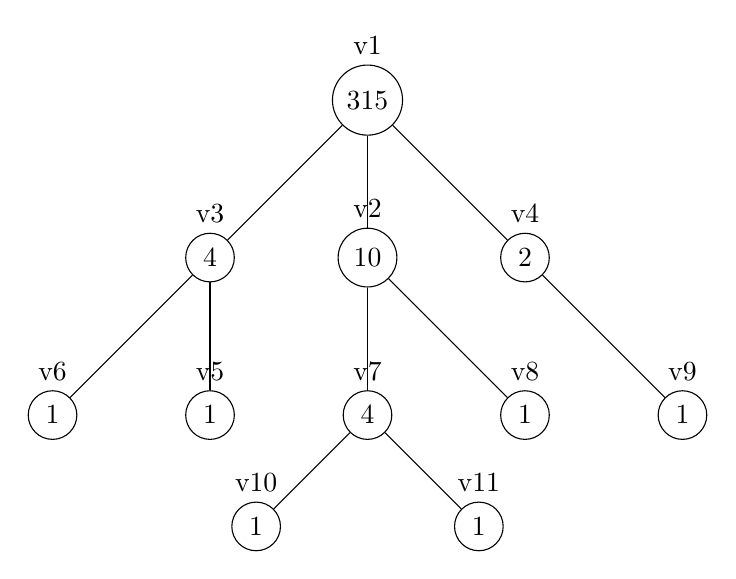
\begin{tikzpicture}[node distance=2cm]
\node[circle,draw,label=v1] (1)[]{315};
\node[circle,draw,label=v2] (3)[below of=1]{10};
\node[circle,draw,label=v3] (2)[left of=3]{4};
\node[circle,draw,label=v4] (4)[ right of=3]{2};
\node[circle,draw,label=v5] (5)[below of=2]{1};
\node[circle,draw,label=v6] (6)[left of=5]{1};
\node[circle,draw,label=v7] (7)[below of=3]{4};
\node[circle,draw,label=v8] (8)[right of=7]{1};
\node[circle,draw,label=v9] (9)[right of=8]{1};
\node[circle,draw,label=v10] (10)[below left of=7]{1};
\node[circle,draw,label=v11] (11)[below right of=7]{1};
\path
	(1) edge node{} (2)
		 edge node{} (3)
		 edge node{} (4)
	(2) edge node{} (5)
		edge node{} (6)
	(3) edge node{} (7)
		edge node{} (8)
	(4) edge node{} (9)
	(7) edge node{} (10)
		edge node{} (11);	
\end{tikzpicture}
\end{minipage}
\begin{minipage}{.2\textwidth}
\centering
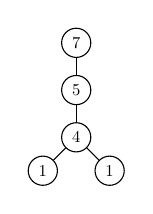
\begin{tikzpicture}[scale=0.1,every node/.style={scale=0.6}]
\node[circle,draw] (5)[]{7};
\node[circle,draw] (1)[below of=5]{5};
\node[circle,draw] (2)[below of=1]{4};
\node[circle,draw] (3)[below left of=2]{1};
\node[circle,draw] (4)[below right of=2]{1};
\path
	(5) edge node{} (1)
	(1) edge node{} (2)
	(2)	 edge node{} (3)
		 edge node{} (4);
\end{tikzpicture}\\Intermediate graph \hfill \\
\begin{tikzpicture}[scale=0.1,every node/.style={scale=0.6}]

\node[circle,draw] (1)[]{3};
\node[circle,draw] (2)[below of=1]{2};
\node[circle,draw] (3)[below of=2]{1};
\path
	(5) edge node{} (1)
	(1) edge node{} (2)
	(2)	 edge node{} (3);
\end{tikzpicture}
\\Intermediate Graph
\end{minipage}
 \caption{NEC based on primes}
\end{figure}
\hspace{10mm}  $v4$ is getting 2 since it has only one child $1$. $v7$ and $v3$ gets 4 since it has two same subgraphs(subgraph $2$) inside them. $v2$ is getting 10 since it has subgraph $2$ and $5$ (see the numbering shown on right). Similiarly $v1$ has two $3$s($v2$ contributes one $3$) ,one $7$ and one $5$.

 \hspace{10mm}	But this was not effective.When we consider the data graph we will need to store only one integer the product of all the graphs inside that node. The first problem we faced was the value of composite number can go beyond the long integer limit. So we tried only storing only primes. But that also didn't make much difference. By our propagation algorithm in Data Graph, we start by giving id $1$ to all nodes in the data graph in the first iteration. In the second iteration every node will get id $2$ since every node will have a child of id $1$. Then in third every node will get $3$ and so on. So every node gets every id present in query graph.
 
 \hspace{10mm} It only helped as in knowing whether there exist a path of length matching the largest length path in query graph. This will lead to all nodes becoming a candidate for the final search we atleast one graph existed in the connected component. So it is not making the CVS tight.
	